% Generado por analysis/src/tablas/figuras_tex.py — no editar a mano.
\begin{figure*}[!tbp]
\centering
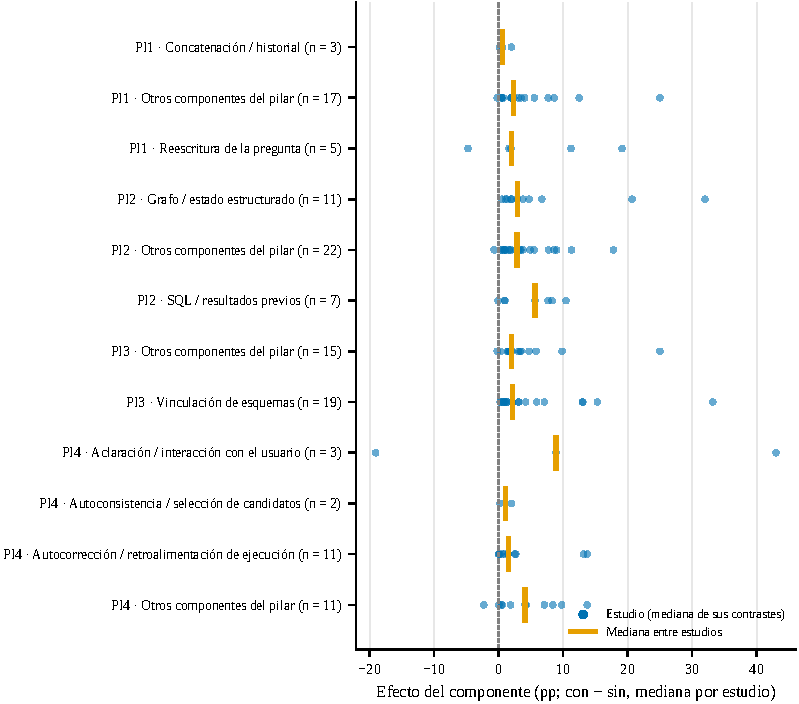
\includegraphics[width=5.33in,height=0.85\textheight,keepaspectratio]{pi_efectos_componentes}
\caption{Efecto de cada clase de componente según los contrastes dentro del estudio (activado frente a desactivado, mismo modelo base y configuración), en puntos porcentuales sobre métricas de exactitud. Cada punto es la mediana de los contrastes de un estudio; la barra, la mediana entre estudios. Síntesis sin metaanálisis (SWiM); estudios del Nivel 2 con validez $\geq$ 50 \%.}
\label{fig:pi_efectos_componentes}
\end{figure*}
